\documentclass[12pt,a4paper]{report}
\usepackage[utf8]{vietnam}
\usepackage[top=2cm, bottom=2cm, left=2cm, right=2cm]{geometry}
\usepackage{amsmath,amsfonts,amssymb}
\usepackage{indentfirst,enumitem}
\usepackage{graphicx}
\usepackage{multicol}
\usepackage{multirow}
\usepackage{longtable}
\usepackage{setspace}
\usepackage{hyperref}
\usepackage{listings}
\usepackage{tabularx}
\usepackage{hyperref}
\usepackage{xcolor}
\usepackage{scrextend}
\usepackage{comment}
\usepackage{soul}
\usepackage{tikz,tkz-tab}
%\changefontsizes{13pt}
\renewcommand\thesection{\Roman{section}}
\renewcommand\thesubsection{\arabic{subsection}}

%New colors defined below
\definecolor{codegreen}{rgb}{0,0.6,0}
\definecolor{codegray}{rgb}{0.5,0.5,0.5}
\definecolor{codepurple}{rgb}{0.58,0,0.82}
\definecolor{backcolour}{rgb}{0.95,0.95,0.92}

%Code listing style named "mystyle"
\lstdefinestyle{mystyle}{
  backgroundcolor=\color{backcolour},   commentstyle=\color{codegreen},
  keywordstyle=\color{blue},
  numberstyle=\tiny\color{codegray},
  stringstyle=\color{codepurple},
  basicstyle=\ttfamily\footnotesize,
  breakatwhitespace=false,         
  breaklines=true,                 
  captionpos=b,                    
  keepspaces=true,                 
  numbers=left,                    
  numbersep=5pt,                  
  showspaces=false,                
  showstringspaces=false,
  showtabs=false,                  
  tabsize=2
}

%"mystyle" code listing set
\lstset{style=mystyle}

\begin{document}
\begin{titlepage}
%\SetWatermarkText{\includegraphics[width = 0.97\paperwidth,
%height = 0.97\paperheight]{bia.png}}
%\SetWatermarkAngle{0} 
%\SetWatermarkText{\includegraphics[scale=1]{hust.png}}
%\SetWatermarkAngle{0} 
\begin{tikzpicture}[remember picture,overlay,inner sep=0,outer sep=0]
     \draw[blue!70!black,line width=4pt] ([xshift=-1.5cm,yshift=-2cm]current page.north east) coordinate (A)--([xshift=1.5cm,yshift=-2cm]current page.north west) coordinate(B)--([xshift=1.5cm,yshift=2cm]current page.south west) coordinate (C)--([xshift=-1.5cm,yshift=2cm]current page.south east) coordinate(D)--cycle;

     \draw ([yshift=0.5cm,xshift=-0.5cm]A)-- ([yshift=0.5cm,xshift=0.5cm]B)--
     ([yshift=-0.5cm,xshift=0.5cm]B) --([yshift=-0.5cm,xshift=-0.5cm]B)--([yshift=0.5cm,xshift=-0.5cm]C)--([yshift=0.5cm,xshift=0.5cm]C)--([yshift=-0.5cm,xshift=0.5cm]C)-- ([yshift=-0.5cm,xshift=-0.5cm]D)--([yshift=0.5cm,xshift=-0.5cm]D)--([yshift=0.5cm,xshift=0.5cm]D)--([yshift=-0.5cm,xshift=0.5cm]A)--([yshift=-0.5cm,xshift=-0.5cm]A)--([yshift=0.5cm,xshift=-0.5cm]A);


     \draw ([yshift=-0.3cm,xshift=0.3cm]A)-- ([yshift=-0.3cm,xshift=-0.3cm]B)--
     ([yshift=0.3cm,xshift=-0.3cm]B) --([yshift=0.3cm,xshift=0.3cm]B)--([yshift=-0.3cm,xshift=0.3cm]C)--([yshift=-0.3cm,xshift=-0.3cm]C)--([yshift=0.3cm,xshift=-0.3cm]C)-- ([yshift=0.3cm,xshift=0.3cm]D)--([yshift=-0.3cm,xshift=0.3cm]D)--([yshift=-0.3cm,xshift=-0.3cm]D)--([yshift=0.3cm,xshift=-0.3cm]A)--([yshift=0.3cm,xshift=0.3cm]A)--([yshift=-0.3cm,xshift=0.3cm]A);

   \end{tikzpicture}
\begin{center}
    \vspace{7pt}
    
    \textbf{ĐẠI HỌC QUỐC GIA THÀNH PHỐ HỒ CHÍ MINH}
    
    \vspace{7pt}
    \textbf{TRƯỜNG ĐẠI HỌC BÁCH KHOA}
\end{center}
\vspace{10pt}
\begin{center}
    
\includegraphics[scale=0.3]{HCMUT.png}
    
    \vspace{10pt}
    \fontsize{18pt}{17pt}\selectfont 
    \textbf{BÁO CÁO THÍ NGHIỆM} 
    
    \vspace{7pt}
    \textbf{HÓA ĐẠI CƯƠNG}
\end{center}

\begin{center}
    \vspace{15pt}
\textbf{Lớp: L38}
\end{center}

\begin{center}
    \vspace{15pt}
\textbf{GVHD: Võ Nguyễn Lam Uyên}
\end{center}

\begin{center}
\vspace{15pt}
\textbf{Nhóm: 03}
\end{center}

\vspace{10pt}
\textbf{DANH SÁCH THÀNH VIÊN:}
    \begin{tabbing}
\hspace{8cm}\=\hspace{3cm}\=\hspace{3cm} \kill
{\it \textbf{Họ và tên}}\>{\it \textbf{MSSV}}\>{\it \textbf{Ghi chú}}\\
\begin{bfseries}Vũ Nhật Huy \end{bfseries}\> \begin{bfseries}2311267 \end{bfseries}\> \begin{bfseries} \end{bfseries}\\
\begin{bfseries}Nguyễn Quốc Huy \end{bfseries}\> \begin{bfseries}2311213 \end{bfseries}\> \begin{bfseries} \end{bfseries}\\
\end{tabbing}

\vfill
\centerline{\bf Thành phố Hồ Chí Minh - 2024}
\vspace{1cm}
\end{titlepage}
\onehalfspacing
\newpage

\tableofcontents
\thispagestyle{empty}
\newpage
\section{Lời nói đầu}
Thí nghiệm luôn là một trong những môn học cần thiết trong quá trình học tập để kiểm tra năng lực kiến thức và khả năng thực hành của bản thân, giúp rèn luyện khả năng tư duy và năng lực sáng tạo của sinh viên trong quá trình thực nghiệm. Tại trường ĐH Bách Khoa ĐHQG TPHCM, THÍ NGHIỆM HÓA ĐẠI CƯƠNG là môn học quan trọng với các sinh viên thuộc khối ngành kĩ thuật nhằm trang bị những kiến thức cơ bản, kĩ năng thực hành trong phòng thí nghiệm, đồng thời giúp sinh viên hiểu rõ các hiện tượng trong các phản ứng hóa học, việc được chiêm ngưỡng tận mắt những màu sắc muôn màu trong các ống nghiệm, các bình thủy phân sẽ giúp sinh viên có cái nhìn khách quan về môn học, chứ không cảm thấy sự khô khan khi chỉ học trên sách vở. Dù mới được thực hành khoảng 4 tuần nhưng chúng em cũng đã được làm quen với các dụng cụ thí nghiệm và các bài thí nghiệm cơ bản. Những điều ấy đã kích thích sự tìm tòi và say mê của chúng em, chúng em đã có những trải nghiệm tuyệt vời trong phòng thí nghiệm. 

Được sự phân công của giảng viên bộ môn, cùng với những kiến thức tích lũy được trong quá trình học tập, chúng em xin trình bày các bài thí nghiệm số 1, 2, 4 và 8. Qua việc thực hiện bài báo cáo này, nhóm chúng em đã biết thêm rất nhiều kiến thức mới lạ và bổ ích. Do vốn kiến thức của chúng em vẫn còn hạn chế nên mặc dù đã cố gắng hết sức nhưng chắc chắn khó tránh khỏi những thiếu sót. Kính mong cô xem xét, góp ý để bài báo cáo của chúng em được hoàn thiện hơn. Ở bài báo cáo lần này, mặc dù đã dành nhiều thời gian chỉnh sửa, nhưng chắc chắn chúng em không thể tránh khỏi thiếu sót. Vì thế, nhóm chúng em mong nhận được sự góp ý, động viên từ cô để có thể hoàn thiện hơn, xin chân thành cảm ơn cô!
\newpage
\section{Bài 1: Kỹ thuật phòng thí nghiệm}
    \subsection{Giới thiệu}

\textbf{Dụng cụ chứa hóa chất:} cốc thủy tin (becher), bình tam giác (erlen), bình cầu. 

\textbf{Dụng cụ lấy hóa chất:} burret, pipet bầu (10ml), pipet vạch, bình định mức, ống đong, phễu nhựa, pipet nhựa.
\subsection{Tiến trình thí nghiệm}
    \subsection*{Thí nghiệm 1: Cách sử dụng pipet.}

        \begin{itemize}
            \item Dùng 10 ml lấy 10 ml nước từ becher cho vào erlen (hút nước bằng quả bóp cao su).
            \item Lặp lại phần thực hành trên. 
        \end{itemize}
    \subsection* {Thí nghiệm 2: Cách sử dụng buret.}

   
        \begin{itemize}
            \item Dùng becher 50ml cho nước vào buret.
            \item Chờ đến khi không còn sủi bọt khí sót lại.
            \item Dùng tay trái mở nhanh khóa buret sao cho dung dịch lấp đầy phần cuối buret.
            \item Chỉnh buret đến mức 0.
            \item Dùng tay trái điều chỉnh khóa buret để 10ml nước từ buret vào becher.
        \end{itemize}
\subsection* {Thí nghiệm 3: Chuẩn độ oxy hóa - khử.}

  
        \begin{itemize}
            \item Cân 0,9g axit oxalic, hòa tan bằng nước cất thành 100ml dung dịch axit oxalic. Đổ dung dịch mới pha vào becher.
            \item Dùng pipet 10ml lấy 10ml dung dịch axit oxalic trên cho vào erlen. Thêm 2ml dung dịch $H_2SO_4$ 1N.
            \item Dùng buret chứa dung dịch $KMnO_4$ 0,1N.
            \item Nhỏ từ từ dung dịch $KMnO_4$ vào erlen trên, lắc đều cho đến khi dung dịch trong erlen có màu tím nhạt. Đọc thể tích $KMnO_4$ đã sử dụng. Viết phương trình phản ứng tổng quát. Tính nồng độ axit oxalic. Biết phương trình ion rút gọn: \[2MnO_4^- + 5C_2O_4^{2-} + 16H^+ \rightarrow 2Mn^{2+} + 10CO_2+ 8H_2O\]
            \item Xác định chất oxi hóa - khử trong phản ứng trên, biết: \[\varphi^0\thickspace MnO_4^- /Mn^{2+} = 1,51V,\thickspace  \varphi^0 \thickspace 2CO_2/C_2O_4^{2-} = -0,49V\]
        \end{itemize}
 \subsection* {Thí nghiệm 4: Pha loãng dung dịch.}  
  
        \begin{itemize}
            \item Dùng pipet bầu lấy 10ml dung dịch HCl 1M cho vào bình định mức 100ml.
            \item Thêm nước vào gần đến vạch trên cổ bình định mức bằng ống đong.
            \item Dùng bình tia cho từng giọt nước đến vạch. 
            \item Đậy nút bình và lắc đều. Ta thu được 100ml dung dịch HCl 0,1M. 
        \end{itemize}
 \subsection* {Thí nghiệm 5: Kiểm tra nồng độ axit đã pha loãng.}  

    
        \begin{itemize}
            \item Tráng buret bằng nước cất, sau đó tráng lại bằng NaOH 0,1M. 
            \item Cho dung dịch NaOH 0,1M vào buret, chuẩn đến vạch 0. 
            \item Dùng pipet 10ml cho vào erlen 10ml dung dịch HCl 0,1M vừa pha xong.
            \item Thêm 1 giọt chỉ thị Phenolphtalein, lắc nhẹ. 
            \item Cho từ từ NaOH từ buret vào erlen, vừa cho vừa lắc đều cho đến khi dung dịch chuyển sang hồng nhạt bền thì dừng lại. 
            \item Đọc thể tích NaOH đã dùng trên buret.
            \item Tính lại nồng độ dung dịch axit vừa pha loãng. 
            \item Lặp lại 2 lần để tính giá trị trung bình.
        \end{itemize}
\newpage
\section{Bài 2: Nhiệt phản ứng}
%%%%%%%%%%%%%%%%%%%%%%%%%%%%%%%%%%%%%%%%%%%%%%%%%  TIẾN TRÌNH
\subsection{Tiến trình thí nghiệm}
\subsection*{Thí nghiệm 1: Xác định nhiệt dung của nhiệt lượng kế:}

Vì công thức tính nhiệt lượng là $Q = mc\Delta t$ trong đó $m$ là khối lượng tất cả các chất được nung nóng hay làm lạnh bao gồm các hoá chất và cả nhiệt lượng kế đựng chúng, do đó công thức trong trường hợp thí nghiệm là:
\begin{equation} \label{eq: 1}
    Q = (m_0 c_0 + mc)\Delta t
\end{equation}
Trong đó:
\begin{itemize}
    \item $m_0 c_0$: nhiệt dung của nhiệt lượng kế (cal/độ)
    \item $mc$: nhiệt dung của dung dịch trong nhiệt lượng kế (cal/độ)
\end{itemize}
Cách bước làm:
\begin{itemize}
    \item[-] Lấy 50ml nước ở nhiệt độ phòng cho vào becher đo nhiệt độ $t_1$.
    \item[-] Lấy 50ml nước khoảng 60℃ cho vào nhiệt lượng kế, để yên 2 phút rồi đo nhiệt độ $t_2$.
    \item[-] Dùng phễu đổ nhanh 50ml ở nhiệt độ phòng vào nhiệt lượng kế chứa 50ml nước và đọc giá trị nhiệt độ $t_3$ đến khi nhiệt độ không đổi
    \item[-] Khi đó: nhiệt độ nước nóng và becher toả ra bằng nhiệt độ nước lạnh hấp thụ.
    \[ (mc + m_0 c_0)(t_2-t_3) = mc(t_3-t_1) \]
    \[ \Rightarrow m_{0} c_0 = mc \frac{(t_3-t_1)-(t_2-t_3)}{(t_2-t_3)} \]
\end{itemize}
Trong đó $m$: khối lượng 50ml nước (g), $c$: nhiệt lượng riêng của nước (1cal/g độ)

\subsection*{Thí nghiệm 2: Xác định hiệu ứng nhiệt của phản ứng trung hoà HCl và NaOH:}

\begin{itemize}
    \item[-] Dùng buret lấy 25 ml dung dịch NaOH 1M cho vào becher 100ml để bên ngoài nhiệt độ phòng. Đo nhiệt độ $t_1$.
    \item[-] Dùng buret lấy 25ml dung dịch HCl 1M cho vào nhiệt lượng kế. Đo nhiệt độ $t_2$.
    \item[-] Dùng phễu đổ nhanh becher chứa dung dịch NaOH vào becher chứa HCl trong nhiệt lượng kế. Khuấy đều dung dịch trong nhiệt lượng kế. Đo nhiệt độ $t_3$.
    \item[-] Xác định $Q$ phản ứng theo công thức \ref{eq: 1} từ đó xác định $\Delta H$.
\end{itemize}

\subsection*{Thí nghiệm 3: Xác định nhiệt hoà tan $CuSO_4$ khan – kiểm tra định luật Hess:}
\begin{comment}
Chúng ta sẽ xác định hiệu ứng nhiệt hoà tan của $CuSO_4$ khan ($\Delta H_3$) bằng thực bghiệm. Lấy vào nhiệt lượng kế 50ml nước. Đo nhiệt độ $t_1$.
Cân chính xác khoảng 4g $CuSO_4$ khan.
Cho nhanh 4g $CuSO_4$ vừa cân nhiệt lượng kế, khuấ
y đều cho $CuSO_4$ tan hết. 
Đo nhiệt độ $t_2$.
Xác định $Q$ theo công thức $Q = (m_0 c_0 + mc)\Delta t$ trong đó:
\begin{itemize}
    \item $m$: khối lượng dung dịch $CuSO_4$ khan.
    \item $c$: nhiệt dung riêng dung dịch $CuSO_4$ (lấygần đúng bằng 1 cal/độ).
\end{itemize}
Từ $Q$ suy ra $\Delta H_{t}$.
\end{comment}
\begin{itemize}
    \item[-] Cho 50ml nước vào nhiệt lượng kế. Đo nhiệt độ $t_1$.
    \item[-] Cân chính xác 4g CuSO$_4$ khan.
    \item[-] Cho nhanh 4g CuSO$_4$ vào nhiệt lượng kế, khuấy đều cho CuSO$_4$ tan hết đo nhiệt độ $t_2$
\end{itemize}
\subsection*{ Xác định nhiệt độ hoà tan của $NH_4Cl$:}

Làm tương tự TN 3 nhưng thay $CuSO_4$ khan bằng $NH_4Cl$. 
%%%%%%%%%%%%%%%%%%%%%%%%%%%%%%%%%%%%%%%%%%%%%%%%%%%%%%%%% KẾT QUẢ
\subsection{Kết quả}
\subsection*{Thí nghiệm 1: Xác định nhiệt dung của nhiệt lượng kế.}

\[
m_0 c_0 = mc \frac{(t_3 - t_1) - (t_2 - t_3)}{(t_2 - t_3)}
\]

Với \( 0 \leq m_0 c_0 \leq 10 \)

Trong đó:
\begin{itemize}
    \item \( m \): khối lượng 50 ml nước
    \item \( c \): nhiệt dung riêng của nước (1 cal/g.độ)
\end{itemize}   
\begin{table}[h!]
    \centering
    \begin{tabular}{|c|c|}
    \hline
    \textbf{Nhiệt độ $^o$C}    & \textbf{Lần 2} \\ \hline
    \textbf{$t_1$}             & $32$           \\ \hline
    \textbf{$t_2$}             & $52$           \\ \hline
    \textbf{$t_3$}             & $42,5$         \\ \hline
    \textbf{$m_0c_0$ (cal/độ)} & $5,3$          \\ \hline
    \end{tabular}
\end{table}
\[
    m_0c_0 = mc\frac{(t_3 - t_1) - (t_2 - t_3)}{(t_2 - t_3)} = 50\times1\times \frac{(42,5 -32)-(52-42,5)}{52-42,5}= 5,3 \text{ (cal/độ)}
\]
\subsection*{Thí nghiệm 2: Xác định hiệu ứng nhiệt của phản ứng trung hòa HCl và NaOH.}
Ta có $Q = (m_0c_0 + mc)\Delta t \Rightarrow Q = (m_0c_0 + mc)(t_3 - t_1)$. Trong đó:
\begin{itemize}
    \item Nhiệt dung riêng của NaCl 0,5M là 1 cal/g.độ
    \item Khối lượng riêng của NaCl là 1,02g/ml.
\end{itemize}
Thể tích của HCl và NaOH bằng 25ml, nồng độ mol là 1M suy ra số mol 2 chất là:
\[ 
    n = C_M V = 0,025 \times 1 = 0,025 (mol)    
\]
Thể tích của phản ứng: $V_{NaOH} + V_{HCl} = 50ml$.\\
Khối lượng dung dịch NaCl: $m_{ddNaCl} = D_{NaCl} \times V = 50 \times 1,02 = 51(g)$.
\[
    \Rightarrow Q = (m_0c_0 + mc)(t_3 - t_1) = (m_0c_0 + mc)\left(t_3 - \dfrac{t_1 + t_2}{2}\right)
\]
\[
    \Delta H = - \frac{Q}{n} = -\frac{Q}{0,025} \thickspace \text{(cal/mol)}
\]
\begin{table}[h!]
    \centering
    \begin{tabular}{|c|cc|}
    \hline
    \textbf{Nhiệt độ $^o$C}              & \multicolumn{1}{c|}{\textbf{Lần 1}} & \textbf{Lần 2} \\ \hline
    \textbf{$t_1$}                       & \multicolumn{1}{c|}{$30,5$}         & $31$           \\ \hline
    \textbf{$t_2$}                       & \multicolumn{1}{c|}{$31$}           & $31$           \\ \hline
    \textbf{$t_3$}                       & \multicolumn{1}{c|}{$36$}           & $37$           \\ \hline
    \textbf{Q (cal)}                     & \multicolumn{1}{c|}{$295,575$}      & $337,8$        \\ \hline
    \textbf{Q$_\text{trung bình}$ (cal)} & \multicolumn{2}{c|}{$316,6875$}                      \\ \hline
    \textbf{$\Delta$ H (cal/mol)}        & \multicolumn{2}{c|}{-12667,5}                        \\ \hline
    \end{tabular}
    \end{table}
\[
    Q = (m_0c_0 + mc)\left(t_3 - \frac{t_1 + t_2}{2}\right)
\]
\[
   \Rightarrow Q= (5,3 + 1,02\times 50)\left(36-\frac{30,5+31}{2}\right) = 295,575 (cal)
\]
\[
    \Delta \text{ H} = -\frac{Q_\text{trung bình}}{n} = - \frac{316,6875}{0,025} = -12667,5 (cal/mol) < 0 \Rightarrow \text{ Phản ứng tỏa nhiệt}
\]
\subsection*{Thí nghiệm 3: Xác định nhiệt hòa tan CuSO$_4$ khan - kiểm tra định luật Hess.}
\[
    Q = (m_0c_0 + m_{H_2O}c_{H_2O} + m_{CuSO_4}c_{CuSO_4})(t_2 - t_1)
\]
\begin{itemize}
    \item[-] Số mol CuSO$_4$ là : $n_\text{CuSO$_4$} = 0,025$ (mol)
    \item[-] Nhiệt dung riêng của CuSO$_4$ và H$_2$O là 1 (cal/g.độ)
    \item[-] $m_\text{H$_2$O} = 50g, m_\text{CuSO$_4$} = 4,05g$
    \item[-] $\Delta$H = $-\dfrac{Q}{n}$
\end{itemize}
\begin{table}[h!]
\centering
\begin{tabular}{|c|cc|}
\hline
\textbf{Nhiệt độ $^o$C}                  & \multicolumn{1}{c|}{\textbf{Lần 1}} & \textbf{Lần 2} \\ \hline
\textbf{$t_1$}                           & \multicolumn{1}{c|}{$32$}           & $32$           \\ \hline
\textbf{$t_2$}                           & \multicolumn{1}{c|}{$38$}           & $37,5$         \\ \hline
\textbf{Q (cal)}                         & \multicolumn{1}{c|}{$356,1$}        & $326,315$      \\ \hline
\textbf{$\Delta$H (cal/mol)}             & \multicolumn{1}{c|}{$-14244$}       & $-13052,6$     \\ \hline
\textbf{$\Delta$H$_\text{tb}$ (cal/mol)} & \multicolumn{2}{c|}{-13648,3}                         \\ \hline
\end{tabular}
\end{table}
\[
    Q = (m_0c_0 + m_{H_2O}c_{H_2O} + m_\text{CuSO$_4$}c_\text{CuSO$_4$})(t_2 - t_1) = (5,3 +50 + 4,05)(38-32)= 356,1 (cal)
\]
\[
    \Delta H = - \frac{Q}{n} = - \frac{356,1}{0,025} = -14244 (cal/mol) 
\]
\[
    \Delta H_\text{tb} = \frac{\Delta H_1 + \Delta H_2}{2} = \frac{-14244 - 13052,6}{2} = -13648,3 (cal/mol)< 0 \Rightarrow \text{ Phản ứng tỏa nhiệt}    
\]
\subsection*{Thí nghiệm 4: Xác định nhiệt độ hòa tan của NH$_4$Cl.}
\[
    Q = (m_0c_0 + m_{H_2O}c_{H_2O} + m_{NH_4Cl}c_{NH_4Cl})(t_2 - t_1)
\]
\begin{itemize}
    \item Số mol NH$_4$Cl là : $n_\text{NH$_4$Cl} = 0,075$ (mol)
    \item Nhiệt dung riêng của NH$_4$Cl và H$_2$O là 1 (cal/g.độ)
    \item m$_\text{H$_2$O}$ = 50g, m$_\text{NH$_4$Cl}$ = 4g
    \item $\Delta$H = $-\dfrac{Q}{n}$
\end{itemize}
\begin{table}[h!]
\centering
\begin{tabular}{|c|cc|}
\hline
\textbf{Nhiệt độ $^o$C}                  & \multicolumn{1}{c|}{\textbf{Lần 1}} & \textbf{Lần 2} \\ \hline
\textbf{m (g)}                           & \multicolumn{1}{c|}{$4,04$}         & $4,02$         \\ \hline
\textbf{$t_1$}                           & \multicolumn{1}{c|}{$32$}           & $32$           \\ \hline
\textbf{$t_2$}                           & \multicolumn{1}{c|}{$28$}           & $27,5$         \\ \hline
\textbf{Q (cal)}                         & \multicolumn{1}{c|}{$-237,36$}      & $-266,94$      \\ \hline
\textbf{$\Delta$H (cal/mol)}             & \multicolumn{1}{c|}{$3164,8$}       & $3559,2$       \\ \hline
\textbf{$\Delta$H$_\text{tb}$ (cal/mol)} & \multicolumn{2}{c|}{3362}                            \\ \hline
\end{tabular}
\end{table}
\[
    Q = (m_0c_0 + m_{H_2O}c_{H_2O} + m_{NH_4Cl}c_{NH_4Cl})(t_2 - t_1) = (5,3 + 50 +4,04)(28-32) = -237,36 (cal)
\]
\[
    \Delta H = - \frac{Q}{n} = - \frac{-237,36}{0,075} = 3164,8 (cal/mol)
\]
\[
    \Delta H_\text{tb} = \frac{\Delta H_1 + \Delta H_2}{2} = \frac{3164,8 + 3559,2}{2} = 3362 (cal/mol) > 0 \Rightarrow \text{ Phản ứng thu nhiệt}    
\]
%%%%%%%%%%%%%%%%%%%%%%%%%%%%%%%%%%%%%%%%%%%%% TRẢ LỜI CÂU HỎI
\subsection{Trả lời câu hỏi}
\noindent\textbf{1. $\Delta H_{tb}$ của phản ứng $HCl + NaOH \rightarrow NaCl + H_2O$ sẽ được tính theo số mol HCl hay NaOH khi cho $25ml$ dung dịch HCl 2M tác dụng với $25ml$ dung dịch NaOH 1M? Tại sao?}

Ta có số mol của NaOH : nNaOH = 0,025 mol 

Số mol của HCl: nHCl = 0,05mol 
\begin{table}[h!]
    \begin{tabular}{lcccc}
                 & \multicolumn{4}{c}{$HCl + NaOH \rightarrow NaCl + H_2O$} \\
    Ban đầu      & 0,05          & 0,025        &             &             \\
    Phản ứng     & 0,025         & 0,025        & 0,025       & 0,025       \\
    Sau phản ứng & 0,0,25        & 0            & 0,025       &            
    \end{tabular}
\end{table}\\
$\rightarrow$ Ta thấy NaOH phản ứng hết và HCl còn dư, nên $\Delta H_{tb}$ của phản ứng tính theo NaOH. Vì lượng dư HCl dư không tham gia phản ứng nên không sinh ra nhiệt. \\
\textbf{2. Nếu thay HCl 1M bằng HNO$_3$ 1M thì kết quả thí nghiệm 2 có thay đổi hay không?}
\begin{itemize}
    \item[+] Nếu thay HCl 1M bằng HNO$_3$ 1M thì kết quả thí nghiệm 2 vẫn không thay đổi vì HNO3 cũng là một axit mạnh phân li hoàn toàn. 
\end{itemize}
\[
    HCl \rightarrow H^+ + Cl^- 
\]
\[
    HNO_3 \rightarrow H^+ + NO_3^- 
\]
\begin{itemize}
    \item[+] Đồng thời thí nghiệm 2 cũng là một phản ứng trung hòa $H^+ + OH^- \rightarrow H_2O$
    \item[+] Sau khi thay công thức $Q=mc\Delta t$ có $m$, $c$ đều có thay đổi, nhưng ở đại lượng $m$, $c$, $\Delta t$ sẽ biến đổi đều cho Q không đổi suy ra $\Delta H$ cũng không đổi. 
\end{itemize}
\textbf{3. Tính $\Delta H_3$ bằng lý thuyết theo định luật Hess. So sánh với kết quả thí nghiệm.}
Hãy xem 6 nguyên nhân có thể gây ra sai số trong thí nghiệm này: 
\begin{itemize}
    \item[-] Mất nhiệt độ do nhiệt lượng kế.
    \item[-] Do nhiệt kế.
    \item[-] Do dụng cụ đong thể tích hóa chất.
    \item[-] Do cân.
    \item[-] Do sunphat đồng bị hút ẩm.
    \item[-] Do lấy nhiệt dung riêng sunphat đồng bằng 1 cal/mol.độ.
\end{itemize}
\textbf{Theo em sai số nào là quan trọng nhất, giải thích? Còn nguyên nhân nào khác không?}
\begin{itemize}
    \item[+] Theo định luật Hess: $\Delta H_3 = \Delta H_1 + \Delta H_2 = -18,7 + 2,8 = -15,9$ (kcal/mol).
    \item[+] Theo thực nghiệm thực tế: $\Delta H_3 = -10,479$ (kcal/mol).
\end{itemize}
Trong 6 nguyên nhân trên, nguyên nhân quan trọng nhất là do Đồng Sunphat ($CuSO_4$) bị hút ẩm. Vì ở điều kiện thường sẽ có lẫn hơi nước nên sẽ có độ ẩm, CuSO$_4$ khan nên sau khi tiếp xúc với không khí, CuSO$_4$ khan sẽ hút ẩm ngay lập tức và tỏa ra một nhiệt lượng đáng kể, khiến ta sai lệch đi giá trị t2 chúng ta đo ở mỗi lần thí nghiệm. 

Theo em còn 2 nguyên nhân khác làm cho kết quả sai số: 
\begin{itemize}
    \item[+] Cân điện tử cân hóa chất chính xác, tuy nhiên lượng chất chúng ta lấy là khác nhau cũng gây ra sự biến đổi nhiệt đáng kể.
    \item[+] Lượng CuSO$_4$ trong phản ứng có thể không tan hết làm mất đi một lượng đáng kể phải được sinh ra trong quá trình hòa tan.
\end{itemize}
\newpage
\section{Bài 4: Xác định bậc phản ứng}
\subsection{Tiến trình thí nghiệm}
\subsection*{Thí nghiệm 1: Xác định bậc phản ứng Na$_2$S$_2$O$_3$:}
\noindent Chuẩn bị 3 ống nghiệm chứa H$_2$SO$_4$ và 3 bình tam giác chứa Na$_2$S$_2$O$_3$ và H$_2$O theo bảng sau:
\begin{center}
\begin{tabular}{|c|c|c|c|}
\hline
TN & Ống nghiệm V(ml) $H_2SO_4$ 0,4M & Erlen V(ml) Na$_2$S$_2$O$_3$ 0,1M & Erlen V(ml) $H_2O$ \\
\hline
1 & 8 & 4 & 28 \\
2 & 8 & 8 & 24 \\
3 & 8 & 16 & 16 \\
\hline
\end{tabular}
\end{center}

\begin{itemize}
    \item[-] Dùng pipet vạch lấy axit cho vào ống nghiệm.
    \item[-] Dùng buret cho H$_2$O vào 3 bình cầu trước, sau đó tráng buret bằng Na$_2$S$_2$O$_3$ 0,1M rồi tiếp tục dùng buret để cho Na$_2$S$_2$O$_3$ vào các bình cầu.
    \item[-] Chuẩn bị đồng hồ bấm giây.
    \item[-] Lần lượt cho phản ứng từng cặp ống nghiệm và bình cầu như sau:
    \begin{itemize}
        \item[+] Đổ nhanh axit trong ống nghiệm vào bình cầu.
        \item[+] Bấm đồng hồ.
        \item[+] Lắc nhẹ bình cầu cho đến khi vừa thấy dung dịch chuyển sang đục thì bấm đồng hồ lần nữa.
        \item[+] Đọc $\Delta t$.
    \end{itemize}
    \item[-] Lặp lại mỗi thí nghiệm 1 lần nữa để lấy giá trị trung bình.
\end{itemize}

\subsection*{Thí nghiệm 2: Xác định bậc phản ứng theo H$_2$SO$_4$:}

Làm tương tự Thí nghiêm 1 với lượng axit và Na$_2$S$_2$O$_3$ theo bảng sau:

\begin{center}
\begin{tabular}{|c|c|c|c|}
\hline
TN & Ống nghiệm V(ml) H$_2$SO$_4$ 0,4M & Erlen V(ml) Na$_2$S$_2$O$_3$ 0,1M & Erlen V(ml) H$_2$O \\
\hline
1 & 4 & 8 & 28 \\
2 & 8 & 8 & 24 \\
3 & 16 & 8 & 16 \\
\hline
\end{tabular}
\end{center}
\newpage
\subsection{Kết quả}
\subsection*{Thí nghiệm 1: Bậc phản ứng theo Na$_2$S$_2$O$_3$.}
\begin{table}[h!]
    \centering
    \begin{tabular}{|c|cc|c|c|c|}
    \hline
    \multirow{2}{*}{\textbf{TN}} & \multicolumn{2}{c|}{\textbf{Nồng độ ban đầu (M)}}                     & \multirow{2}{*}{\textbf{$\Delta t_1$ (s)}} & \multirow{2}{*}{\textbf{$\Delta t_2$ (s)}} & \multirow{2}{*}{\textbf{$\Delta t_{tb}$ (s)}} \\ \cline{2-3}
                                 & \multicolumn{1}{c|}{\textbf{Na$_2$S$_2$O$_3$}} & \textbf{H$_2$SO$_4$} &                                            &                                            &                                            \\ \hline
    \textbf{1}                   & \multicolumn{1}{c|}{0,1}                       & 0,4                  & 104                                        & 108                                        & 106                                        \\ \hline
    \textbf{2}                   & \multicolumn{1}{c|}{0,1}                       & 0,4                  & 46                                         & 48                                         & 47                                        \\ \hline
    \textbf{3}                   & \multicolumn{1}{c|}{0,1}                       & 0,4                  & 23                                         & 24                                         & 23,5                                       \\ \hline
    \end{tabular}
    \end{table}
\noindent Từ $\Delta t_{tb}$ của TN1 và TN2, xác định $m_1$:
\[
    m_1 = \frac{\lg \dfrac{\Delta t_{tb1}}{\Delta t_{tb2}}}{\lg2} = \frac{\lg \dfrac{106}{47}}{\lg2} = 1,173
\]
Từ $\Delta t_{tb}$ của TN2 và TN3, xác định $m_2$:
\[
    m_2 = \frac{\lg \dfrac{\Delta t_{tb2}}{\Delta t_{tb3}}}{\lg2} = \frac{\lg \dfrac{47}{23,5}}{\lg2} = 1
\]
Bậc phản ứng theo Na$_2$S$_2$O$_3$ = $\dfrac{m_1 + m_2}{2} = \dfrac{1,173 + 1}{2} = 1,0865$.
\subsection*{Thí nghiệm 2: Bậc phản ứng theo H$_2$SO$_4$.}
\begin{table}[h!]
    \centering
    \begin{tabular}{|c|cc|c|c|c|}
    \hline
    \multirow{2}{*}{\textbf{TN}} & \multicolumn{2}{c|}{\textbf{Nồng độ ban đầu (M)}}                     & \multirow{2}{*}{\textbf{$\Delta t_1$ (s)}} & \multirow{2}{*}{\textbf{$\Delta t_2$ (s)}} & \multirow{2}{*}{\textbf{$\Delta t_3$ (s)}} \\ \cline{2-3}
                                 & \multicolumn{1}{c|}{\textbf{Na$_2$S$_2$O$_3$}} & \textbf{H$_2$SO$_4$} &                                            &                                            &                                            \\ \hline
    \textbf{1}                   & \multicolumn{1}{c|}{0,1}                       & 0,4                  & 58                                         & 58,26                                      & 58,13                                      \\ \hline
    \textbf{2}                   & \multicolumn{1}{c|}{0,1}                       & 0,4                  & 46                                         & 48                                         & 47                                         \\ \hline
    \textbf{3}                   & \multicolumn{1}{c|}{0,1}                       & 0,4                  & 40                                         & 44                                         & 42                                       \\ \hline
    \end{tabular}
\end{table}
\noindent Từ $\Delta t_{tb}$ của TN4 và TN5, xác định $n_1$:
\[
    n_1 = \frac{\lg \dfrac{\Delta t_{tb4}}{\Delta t_{tb5}}}{\lg2} = \frac{\lg \dfrac{58,13}{47}}{\lg2} = 0,3066 
\]
Từ $\Delta t_{tb}$ của TN5 và TN6, xác định $n_2$:
\[
    n_2 = \frac{\lg \dfrac{\Delta t_{tb5}}{\Delta t_{tb6}}}{\lg2} = \frac{\lg \dfrac{47}{42}}{\lg2} = 0,1623
\]
Bậc phản ứng theo Na$_2$S$_2$O$_3$ = $\dfrac{m_1 + m_2}{2} = \dfrac{0,3066+0,1623}{2} = 0,2345$.
\subsection{Trả lời câu hỏi}
\noindent\textbf{1. Trong thí nghiệm trên, nồng độ của Na$_2$S$_2$O$_3$ và của H$_2$SO$_4$ đã ảnh hưởng thế nào lên vận tốc phản ứng? Viết lại biểu thức tính vận tốc phản ứng. Xác định bậc của phản ứng.}

Nồng độ của Na$_2$S$_2$O$_3$ tỉ lệ thuận với tốc độ phản ứng. Nồng độ của H$_2$SO$_4$ hầu như không ảnh hưởng tới tốc độ phản ứng. 

Biểu thức tính vận tốc: 
\[
    v = k.\lbrack Na_2S_2O_3 \rbrack^m . \lbrack H_2SO_4\rbrack^n
\]
trong đó m,n là hằng số dương được xác định bằng thực nghiệm. $\rightarrow$ Bậc của phản ứng: $m+n = 1,0865 +0,2345 = 1,321.$\\
\textbf{2. Cơ chế của phản ứng trên có thể được viết như sau:} 
\[
    H_2SO_4 + Na_2S_2O_3 \rightarrow Na_2SO_4 + H_2S_2O_3 \quad (1)
\]
\[
    H_2S_2O_3 \rightarrow H_2SO_3 + S \downarrow \quad (2)  
\]
\textbf{Dựa vào kết quả của TN có thể kết luận phản ứng (1) hay (2) là phản ứng quyết định vận tốc phản ứng tức là phản ứng xảy ra chậm nhất không? Tại sao? Lưu ý trong các TN trên, lượng axit H$_2$SO$_4$ luôn luôn dư so với Na$_2$SO$_3$.}
\begin{itemize}
    \item[-] (1) là phản ứng trao đổi ion nên tốc độ phản ứng xảy ra rất nhanh. 
    \item[-] (2) là phản ứng tự oxi hóa khử nên tốc độ phản ứng xảy ra chậm hơn. 
\end{itemize}
Phản ứng (2) quyết định tốc độ phản ứng, là phản ứng xảy ra chậm nhất do bậc của phản ứng (2) là bậc của cả phản ứng.\\
\textbf{3. Dựa trên cơ sở của phương pháp TN thì vận tốc xác định được trong các TN trên được xem là vận tốc trung bình hay vận tốc tức thời?}

Vận tốc xác định bằng thương của biến thiên nồng độ với biến thiên thời gian $(\Delta C/\Delta t)$. Do $\Delta C \approx 0$ (lưu huỳnh có biến thiên nồng độ không đáng kể trong khoảng thời gian $\Delta t$) nên vận tốc trong các TN trên được xem là vận tốc tức thời. \\
\textbf{4. Thay đổi thứ tự cho H$_2$SO$_4$ và Na$_2$S$_2$O$_3$ thì bậc phản ứng có thay đổi hay không, tại sao?} 

Bậc phản ứng không đổi khi thay đổi thức tự cho H$_2$SO$_4$ và Na$_2$S$_2$O$_3$ vì ở cùng nhiệt độ xác định, bậc phản ứng chỉ phụ thuộc vào bản chất của hệ (nồng độ, nhiệt độ, diện tích bề mặt tiếp xúc, áp suất) mà không phụ thuộc vào thứ tự phản ứng. 
\newpage
\section{Bài 8: Phân tích thể tích}
\subsection{Tiến trình thí nghiệm}

\subsection*{Thí nghiệm 1: Xây dựng đường cong chuẩn độ axit mạnh bằng bazơ mạnh}

\begin{center}
\begin{table}[h!]
\resizebox{\columnwidth}{!}{%
\begin{tabular}{|c|c|c|c|c|c|c|c|c|c|c|c|c|c|c|}
\hline
V$_{\text{NaOH}}$ (ml) & 0    & 2    & 4    & 6    & 8    & 9    & 9.2  & 9.4  & 9.6   & 9.8  & 10    & 11    & 12    & 13    \\ \hline
pH                     & 0.96 & 1.14 & 1.33 & 1.59 & 1.98 & 2.38 & 2.56 & 2.73 & 3.336 & 7.26 & 10.56 & 11.70 & 11.97 & 12.01 \\ \hline
\end{tabular}%
}
\end{table}
\end{center}
Dựa trên đường cong chuẩn độ xác định bước nhảy pH từ ... tới ..., điểm tương đương pH = và chất chỉ thị thích hợp phenolphthalein.

\subsection*{Thí nghiệm 2: Chuẩn độ axit - bazơ với thuốc thử phenolphtalein}

\begin{itemize}
    \item[-] Chuẩn độ axit - bazo với thuốc thử phenolphtalein.
    \item[-] Tráng buret bằng dung dịch NaOH 0,1N, sau đó cho từ từ dung dịch NaOH 0,1N vào buret. Chỉnh mức dung dịch ngang vạch 0.
    \item[-] Dùng pipet 10 ml lấy 10 ml dung dịch HCl chưa biết nồng độ cho vào erlen 150 ml, thêm 10 ml nước cất và 2 giọt phenolphtalein.
    \item[-] Mở khóa buret nhỏ từ từ dung dịch NaOH xuống erlen, vừa nhỏ vừa lắc nhẹ đến khi dung dịch trong erlen chuyển sang màu hồng nhạt bền thì khóa buret. Đọc thể tích dung dịch NaOH đã dùng.
    \item[-] Lặp lại thí nghiệm trên một lần nữa để tính giá trị trung bình.
\end{itemize}

\subsection*{Thí nghiệm 3: Chuẩn độ axit mạnh-bazơ mạnh bằng chỉ thị metyl da cam}

\begin{itemize}
    \item[-] Tiến hành như thí nghiệm 2 nhưng thay chất chỉ thị phenolphtalein bằng methyl da cam. Màu dung dịch đổi từ đỏ sang vàng.
\end{itemize}

\subsection*{Thí nghiệm 4: Chuẩn độ axit yếu -bazơ mạnh bằng chỉ thị phenolphtalein + metyl da cam}

\begin{itemize}
    \item[-] Tiến hành như thí nghiệm 2 nhưng thay dung dịch HCl bằng dung dịch axit acetic. Làm thí nghiệm 2 lần với lần đầu dùng chất chỉ thị là phenolphtalein, lần sau dùng methyl da cam.
\end{itemize}
\newpage
\subsection{Kết quả}
\subsection*{Thí nghiệm 1:} 
\begin{itemize}
 \item[-] Xác định đường cong chuẩn độ HCl bằng NaOH
    \begin{center}
         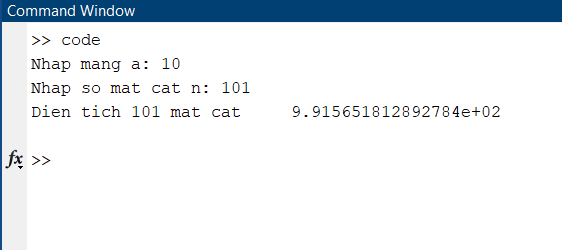
\includegraphics[width=0.7\textwidth]{image.png}
    \end{center}
\item Bước nhảy pH từ pH = 3,36 đến pH = 10,56.
\item Điểm tương đương pH = 7,26.
\item Chất chỉ thị phù hợp: phenolphthalein.
\end{itemize}
\subsection*{Thí nghiệm 2:} 
\begin{table}[h!]
    \centering
    \begin{tabular}{|c|c|c|c|c|c|}
    \hline
    \textbf{Lần} & \textbf{V$_\text{HCl}$ (ml)} & \textbf{V$_\text{NaOH}$ (ml)} & \textbf{C$_\text{NaOH}$ (N)} & \textbf{C$_\text{HCl}$ (N)} & \textbf{Sai số} \\ \hline
    \textbf{1}   & 10                           & 10,5                          & 0,1                          & 0,105                       & 0,0007          \\ \hline
    \textbf{2}   & 10                           & 10,6                          & 0,1                          & 0,106                       & 0,0003          \\ \hline
    \textbf{3}   & 10                           & 10,6                          & 0,1                          & 0,106                       & 0,0003          \\ \hline
    \end{tabular}
    \end{table}
\[
    C_\text{HCl (1)} = \frac{C_\text{NaOH (1)}.V_\text{NaOH (1)}}{V_\text{HCl (1)}} = \frac{0,1.10,5}{10} = 0,105 (N)
\]
\[
    C_\text{HCl (2)} = \frac{C_\text{NaOH (2)}.V_\text{NaOH (2)}}{V_\text{HCl (2)}} = \frac{0,1.10,6}{10} = 0,106 (N)
\]
\[
    C_\text{HCl (3)} = \frac{C_\text{NaOH (3)}.V_\text{NaOH (3)}}{V_\text{HCl (3)}} = \frac{0,1.10,6}{10} = 0,106 (N)
\]
\[
    \Rightarrow C_\text{HCl tb} = \frac{C_\text{HCl (1)}+C_\text{HCl (2)}+C_\text{HCl (3)}}{3} = \frac{0,105 + 0,106+0,106}{3} = 0,1057 (N)
\]
\[
    \Delta C_\text{HCl (1)} = |C_\text{HCl tb} - C_\text{HCl (1)}| = |0,1057 - 0,105| = 0,0007 (N)
\]
\[
    \Delta C_\text{HCl (2)} = |C_\text{HCl tb} - C_\text{HCl (2)}| = |0,1057 - 0,106| = 0,0003 (N)
\]
\[
    \Delta C_\text{HCl (3)} = |C_\text{HCl tb}- C_\text{HCl (3)}| = |0,1057 - 0,106| = 0,0003 (N)
\]
\[
    \Rightarrow \Delta C_\text{HCl tb} = \frac{\Delta C_\text{HCl (1)}+\Delta C_\text{HCl (2)}+\Delta C_\text{HCl (3)}}{3} = \frac{0,0007 +0,0003 + 0,0003}{3} = 0,0004
\]
Kết luận: \( \overline{\text{C}}_{\text{HCl}} \approx 0.1057; \overline{N} \approx 0.0004 \)

\subsection*{Thí nghiệm 3:}
\begin{table}[h!]
\centering
    \begin{tabular}{|c|c|c|c|c|c|}
    \hline
    \textbf{Lần} & \textbf{V$_\text{HCl}$ (ml)} & \textbf{V$_\text{NaOH}$ (ml)} & \textbf{C$_\text{NaOH}$ (N)} & \textbf{C$_\text{HCl}$ (N)} & \textbf{Sai số} \\ \hline
    \textbf{1}   & 10                           & 10,4                          & 0,1                          & 0,104                       & 0,0007          \\ \hline
    \textbf{2}   & 10                           & 10,3                          & 0,1                          & 0,103                       & 0,0003          \\ \hline
    \textbf{3}   & 10                           & 10,3                          & 0,1                          & 0,103                       & 0,0003          \\ \hline
    \end{tabular}
    \end{table}
    \[
        C_\text{HCl (1)} = \frac{C_\text{NaOH (1)}.V_\text{NaOH (1)}}{V_\text{HCl (1)}} = \frac{0,1.10,4}{10} = 0,104 (N)
    \]
    \[
        C_\text{HCl (2)} = \frac{C_\text{NaOH (2)}.V_\text{NaOH (2)}}{V_\text{HCl (2)}} = \frac{0,1.10,3}{10} = 0,103 (N)
    \]
    \[
        C_\text{HCl (3)} = \frac{C_\text{NaOH (3)}.V_\text{NaOH (3)}}{V_\text{HCl (3)}} = \frac{0,1.10,3}{10} = 0,103 (N)
    \]
    \[
        \Rightarrow C_\text{HCl tb} = \frac{C_\text{HCl (1)}+C_\text{HCl (2)}+C_\text{HCl (3)}}{3} = \frac{0,104 + 0,103+0,103}{3} = 0,1033 (N)
    \]
    \[
        \Delta C_\text{HCl (1)} = |C_\text{HCl tb} - C_\text{HCl (1)}| = |0,1033 - 0,104| = 0,0007 (N)
    \]
    \[
        \Delta C_\text{HCl (2)} = |C_\text{HCl tb} - C_\text{HCl (2)}| = |0,1033 - 0,103| = 0,0003 (N)
    \]
    \[
        \Delta C_\text{HCl (3)} = |C_\text{HCl tb}- C_\text{HCl (3)}| = |0,1033 - 0,103| = 0,0003 (N)
    \]
    \[
        \Rightarrow \Delta C_\text{HCl tb} = \frac{\Delta C_\text{HCl (1)}+\Delta C_\text{HCl (2)}+\Delta C_\text{HCl (3)}}{3} = \frac{0,0007 +0,0003 + 0,0003}{3} = 0,0004
    \]
\subsection*{Thí nghiệm 4a:}
\begin{table}[h!]
\centering
    \begin{tabular}{|c|c|c|c|c|c|}
    \hline
    \textbf{Lần} & \textbf{V$_\text{CH3COOH}$ (ml)} & \textbf{V$_\text{NaOH}$ (ml)} & \textbf{C$_\text{NaOH}$ (N)} & \textbf{C$_\text{CH3COOH}$ (N)} & \textbf{Sai số} \\ \hline
    \textbf{1}   & 10                               & 10,2                          & 0,1                          & 0,102                           & 0,0005          \\ \hline
    \textbf{2}   & 10                               & 10,1                          & 0,1                          & 0,101                           & 0,0005          \\ \hline
    \end{tabular}
    \end{table}
    \[
        C_\text{CH$_3$COOH (1)} = \frac{C_\text{NaOH (1)}.V_\text{NaOH (1)}}{V_\text{CH$_3$COOH (1)}} = \frac{0,1.10,2}{10} = 0,102 (N)
    \]
    \[
        C_\text{CH$_3$COOH (2)} = \frac{C_\text{NaOH (2)}.V_\text{NaOH (2)}}{V_\text{CH$_3$COOH (2)}} = \frac{0,1.10,1}{10} = 0,101 (N)
    \]
    \[
        \Rightarrow C_\text{CH$_3$COOH tb} = \frac{C_\text{CH$_3$COOH (1)}+C_\text{CH$_3$COOH (2)}}{2} = \frac{0,102 + 0,101}{2} = 0,1015 (N)
    \]
    \[
        \Delta C_\text{CH$_3$COOH (1)} = |C_\text{CH$_3$COOH tb} - C_\text{CH$_3$COOH (1)}| = |0,1015 - 0,102| = 0,0005 (N)
    \]
    \[
        \Delta C_\text{CH$_3$COOH (2)} = |C_\text{CH$_3$COOH tb} - C_\text{CH$_3$COOH (2)}| = |0,1015 - 0,101| = 0,0005 (N)
    \]
    \[
        \Rightarrow \Delta C_\text{CH$_3$COOH tb} = \frac{\Delta C_\text{CH$_3$COOH (1)}+\Delta C_\text{CH$_3$COOH (2)}}{2} = \frac{0,0005 +0,0005}{2} = 0,0005
    \]
\subsection*{Thí nghiệm 4b.}
\begin{table}[h!]
\centering
    \centering
    \begin{tabular}{|c|c|c|c|c|c|}
    \hline
    \textbf{Lần} & \textbf{V$_\text{CH3COOH}$ (ml)} & \textbf{V$_\text{NaOH}$ (ml)} & \textbf{C$_\text{NaOH}$ (N)} & \textbf{C$_\text{CH3COOH}$ (N)} & \textbf{Sai số} \\ \hline
    \textbf{1}   & 10                               & 4,1                           & 0,1                          & 0,041                           & 0,0005          \\ \hline
    \textbf{2}   & 10                               & 4,2                           & 0,1                          & 0.042                           & 0,0005          \\ \hline
    \end{tabular}
    \end{table}
    \[
        C_\text{CH$_3$COOH (1)} = \frac{C_\text{NaOH (1)}.V_\text{NaOH (1)}}{V_\text{CH$_3$COOH (1)}} = \frac{0,1.4,1}{10} = 0,041 (N)
    \]
    \[
        C_\text{CH$_3$COOH (2)} = \frac{C_\text{NaOH (2)}.V_\text{NaOH (2)}}{V_\text{CH$_3$COOH (2)}} = \frac{0,1.4,2}{10} = 0,042 (N)
    \]
    \[
        \Rightarrow C_\text{CH$_3$COOH tb} = \frac{C_\text{CH$_3$COOH (1)}+C_\text{CH$_3$COOH (2)}}{32} = \frac{0,041 + 0,042}{2} = 0,0415 (N)
    \]
    \[
        \Delta C_\text{CH$_3$COOH (1)} = |C_\text{CH$_3$COOH tb} - C_\text{CH$_3$COOH (1)}| = |0,0415 - 0,041| = 0,0005 (N)
    \]
    \[
        \Delta C_\text{CH$_3$COOH (2)} = |C_\text{CH$_3$COOH tb} - C_\text{CH$_3$COOH (2)}| = |0,0415 - 0,042| = 0,0005 (N)
    \]
    \[
        \Rightarrow \Delta C_\text{CH$_3$COOH tb} = \frac{\Delta C_\text{CH$_3$COOH (1)}+\Delta C_\text{CH$_3$COOH (2)}}{2} = \frac{0,0005 +0,0005}{2} = 0,0005
    \]
\subsection{Trả lời câu hỏi}
\noindent\textbf{1. Khi thay đổi nồng độ HCl và NaOH, đường cong chuẩn độ có thay đổi hay không, tại sao?}

Thay đổi nồng độ HCl và NaOH thì đường cong chuẩn độ không thay đổi vì đương lượng phản ứng của các chất vẫn không thay đổi, chỉ có bước nhảy là thay đổi và điểm pH tương đương vẫn không thay đổi. Nếu dùng nồng độ nhỏ thì bước nhảy nhỏ và ngược lại. \\
\textbf{2. Việc xác định nồng độ axit HCl trong các thí nghiệm 2 và 3 cho kết quả nào chính xác hơn, tại sao? }

Xác định nồng độ axit HCl trong thí nghiệm 2 cho kết quả chính xác hơn. Vì phenolphtalein giúp ta xác đinh màu chính xác hơn, rõ ràng hơn, do chuyển từ không màu sang hồng nhạt, dễ nhận thấy hơn từ màu đỏ sang màu da cam. \\
\textbf{3. Từ kết quả thí nghiệm 4, việc xác định nồng độ dung dịch axit axetic bằng chỉ thị màu nào chính xác hơn, tại sao?}

Phenolphtalein giúp ta xác định chính xác hơn vì pH chuyển màu của phenolphtalein khoảng từ 8-10, nhưng pH chuyển màu của Metyl da cam là 3.1- 4.4. Với thí nghiệm cho Axit yếu tác dụng với Bazo mạnh (CH3COOH tác dụng NaOH), điểm pH tương đương không còn xấp xỉ 7 mà lớn hơn 7 tương đối nhiều, lí do là muối của phản ứng được tạo thành là muối giữa axit yếu và bazo mạnh nên có tính bazo. Bên cạnh đó, bước nhảy pH cũng thay đổi dẫn đến pH chuyển màu của Metyl da cam không còn nằm trong bước nhảy pH nữa, cho nên chúng ta không dùng được Metyl da cam làm chất chỉ thị. Một lý do nữa là vì Phenolphtalein giúp chúng ta xác định màu tốt hơn, rõ ràng hơn. Do từ màu trắng sang hồng nhạt, dễ nhận thấy hơn màu đỏ sang vàng cam. \\
\textbf{4. Trong phép phân tích thể tích nếu đổi vị trí của NaOH và axit thì kết quả có thay đổi không, tại sao? }

Trong phép phân tích thể tích nếu đổi vị trí NaOH và axit thỉ kết quả vẫn không thay đổi vì bản chất phản ứng không thay đổi, vẫn là phản ứng trung hòa và chất chỉ thị cũng sẽ đổi màu tại điểm tương đương.  

\end{document}